\documentclass[12pt]{article}


\usepackage{verbatim}   % useful for program listings
\usepackage{color}      % use if color is used in text
\usepackage{subfigure}  % use for side-by-side figures
\usepackage{hyperref}   % use for hypertext links, including those to external documents and URLs
\usepackage{bigints}
\usepackage{graphicx}

\usepackage[utf8x]{inputenc}
\usepackage[L7x]{fontenc}
\usepackage[lithuanian]{babel}

% above is the preamble

\begin{document}

\begin{center}
{\large Atsitiktiniu vektorių generavimas} \\ % \\ = new line
Lukas Klusis \\
2014 birželio 20 d.
\end{center}

\section{Įvadas}
Yra žinoma daugybė variantų, kaip generuoti 1-dimensijos (pseudo) atsitiktinius skaičius. Turbūt populiariausi yra Tiesinis kongruentinis bei Tiesinis rekurentinis metodai, kurie leidžia mums gauti norimo ilgio tolygiai pasiskirsčiusių atsitiktinių skaičių seką greitai ir efektyviai. Tačiau dažnai neužtenka 1-dimensijos skaičių. Šie metodai taip pat taikomi norint gauti n-dimensijų vektorius, tačiau reikia papildomų veiksmų ir sąlygų. Generuojant atsitiktinį vektorių svarbu atsižvelgti į šio vektoriaus individualių kintamųjų koreliaciją. 
Yra žinoma, jeigu $\xi= (\xi_1, \xi_2, \ldots, \xi_n)$ yra atsitiktinis skaičius, su pasiskirstymo funkcija $G(x_1, x_2, \ldots, x_n) = P\{\xi_1<x_1, \xi_2<x_2, \ldots, \xi_n<x_n\}$, tai ji gali būti išskaidyta į dvi pasiskirstymo funkcijas:
\begin{equation}
\label{eq:pasiskirstymo}
G(x_1, x_2, \ldots, x_n) = G_1(x_1)G_{2\ldots n}(x_2, \ldots, x_n| x_1)
\end{equation}
kur $G_1$ yra pirmosios komponentės besąlygiška pasiskirstymo funkcija, o $G_{2 \ldots n}$ yra sąlygiškai pasiskirsčiusi funkcija komponenčių $x_2, \ldots, x_n$ su sąlyga $x_1 = \xi_1$. Pritaikius šią idėją funkcijai $G_{2 \ldots n}$ ir paėmus \eqref{eq:pasiskirstymo} lygybės dešinę pusę, po $(n-1)$ karto mes išskaidytume šią funkciją tokiu būdu:
\begin{equation}
\begin{split}
\label{eq:išskaidytaPasiskirstymo}
G(x_1, x_2, \ldots, x_n) = G_1(x_1)G_2(x_2| x_1)G_3(x_3| x_1, x_2) \\
\ldots G_n(x_n| x_1, x_2, \ldots x_{n-1})
\end{split}
\end{equation}
kur $G_i(x_i| x_1, x_2, \ldots x_{i-1})$ yra vektoriaus $\xi$ nario $\xi_i$ sąlyginio pasiskirstymo funkcija. Pasinaudoję \eqref{eq:išskaidytaPasiskirstymo} lygtimi galime sukonstruoti bendrą procedūra, kuri generuoti atsitiktinius vektorius su pasiskirstymo funkcija $G(x_1, x_2, \ldots, x_n)$:\\

{\bf Vektoriaus generavimas atitinkantis pasiskirstymo funkciją:}

\begin{enumerate}
	
	\item Generuojame reikšmę $z_1$, tokią kad atitiktų pasiskirstymo funkciją $G_1(x_1)$ ir nustatome kintamąjį $i \longleftarrow 2$
	
	\item Generuojame skaičių $z_i$ pagal sąlyginę pasiskirstymo funkciją \\ $G_i(x_i | x_1=z_1, \ldots x_{i-1} = z_{i-1})$.
	
	\item Jeigu $n>i$, tai padidiname $i$ reikšmę vienetu $i \longleftarrow i+1$ ir grįžtame į Žingsnį 2.
	
	\item Gauname vektorių $(z_1,z_2, \ldots, z_n)$, kuris yra pasiskirstęs pagal pasiskirstymo funkciją $G(x_1, x_2, \ldots, x_n)$.
	
\end{enumerate}


Naudojantis panašiu principu, šio darbo tikslas bus suprasti ir pademonstruoti kaip galima standartizuoti atsitiktinių vektorių generavimą. Arba tiksliau tariant, nagrinėsime kaip reikia generuoti vektorius pasiskirsčiusius pagal Normalųjį skirstinį.


\section{Reikšmės pasiskirsčiusios pagal normalųjį dydį}

Iš pradžių mums reikia išnagrinėti kaip galima generuoti 1-dimensijos atsitiktinius skaičius, kurie būtų pasiskirstę pagal normalųjį dydį, t.y. generuojamos sekos pasiskirstymo funkcija $G(x)$ atitiktų funkciją $\Phi(x) = \dfrac{1}{\sqrt{2\pi}} \bigintss_{-\infty}^x \mathrm{e}^{-\frac{t^2}{2}}\,\mathrm{d}t $
Naudokimės tokiu algoritmu:\\


{\bf \label{alg:norm1} Normaliai pasiskirsčiusio atsitiktinio dydžio gavimas}

\begin{enumerate}
	
	\item Generuojame $u_1$ ir $u_2$, kur $u_1$ ir $u_2$ yra nepriklausomi ir tolygiai pasiskirstę intervale $[0,1)$ atsitiktiniai dydžiai.
	
	\item Apskaičiuojame dydžius $v_1=2u_1-1$ ir $v_2=2u_2-1$, t.y. gauname nepriklausomus atsitiktinius dydžius pasiskirsčiusius intervale $[-1,1)$
	
	\item Apskaičiuojame reikšmę:
	\begin{equation}
	s=v_1^2 + v_2^2.
	\end{equation} 
	
	\item Jeigu $S \geq 1$ grįžtame į Žingsnį 1. Priešingu atveju jeigu $ 0\leq S < 1$ tai tęsiame toliau.
	
	\item Apskaičiuojame dydžius:
	\begin{equation}
	x_1=v_1 \sqrt{\dfrac{-2 \ln{s}}{s}}, x_2=v_2 \sqrt{\dfrac{-2 \ln{s}}{s}}
	\end{equation}
	
	gauti dydžiai $x_1$ ir $x_2$ yra nepriklausomi ir normaliai pasiskirstę atsitiktiniai dydžiai, t.y. $x_1, x_2 \in \mathcal{N}(0,1) $ 
\end{enumerate}


{\bf Įrodymas: \footnote{Pagal G. Stepanausko pateiktą mokomąją medžiagą „Monte Karlo Metodas”, 2008 \cite[p.~70]{STEPANAUSKAS} }}
Pereikime prie polinių koordinačių

\begin{equation}
\begin{split}
v_1 = r \cos{\theta}, v2=r\sin{\theta} \\
\Rightarrow s=r^2\\
\Rightarrow x_1 = \sqrt{-2\ln{s}}\cos \theta, \space x_2 = \sqrt{-2\ln{s}}\sin \theta
\end{split} \nonumber
\end{equation}
Pažymėkime
\begin{equation}
r'=\sqrt{-2 ln{s}} \nonumber
\end{equation}

Dydžiai $r$ ir $\theta$ yra nepriklausomi atsitiktiniai dydžiai, kintantys vienetinio skritulio viduje, nes $v_1$ ir $v_2$ nepriklausomi. Tuomet $r'$ ir $\theta$ taip pat nepriklausomi dydžiai. Tikimybė patekti taškui į vienodo kampo skritulio išpjovas vienoda, todėl $\theta$ yra tolygiai pasiskirstęs intervale $[0,2\pi)$.

Tikimybė
\begin{equation}
\begin{split}
P(r' < R) = P(\sqrt{-2 ln{s}}<R) = P(-2 ln{S} < R^2)\\
= P(ln{S} > - \dfrac{R^2}{2}) = P(S > e^{-\frac{R^2}{2}}) = P(r^2 > e^{-\frac{R ^2}{2}})\\
=1 - P(r^2 \leq e^\frac{R^2}{2})=1-e^{-\frac{R^2}{2}}
\end{split} \nonumber
\end{equation}

nes dydis $r^2$ yra tolygiai pasiskirstęs intervale [0,1). Tai galima įsitikinti, paskaičiavus geometrinę tikimybę:

\begin{equation}
P(r^2 < t) = P(r < \sqrt{t}) = \dfrac{\textnormal{skritulio, su spinduliu $\sqrt{t}$, plotas}}{\textnormal{skritulio, su spinduliu 1, plotas}} = \dfrac{\pi t}{\pi} = t \nonumber
\end{equation}

Taigi atsitiktinio dydžio $r'$ pasiskirstymo funkcija 
\begin{equation}
F_{r'}(R):=P(r' < R) = 1 - e^{-\frac{R^2}{2}}, \space r \geq 0. \nonumber
\end{equation}
Jau minėjome, kad dydis $\theta$ tolygiai pasiskirstęs intervale $[0,2\pi)$, todėl jo pasiskirstymo funkcija 
\begin{equation}
F_\theta(\varphi):=(\theta < \varphi) = \frac{\varphi}{2\pi}, \space 0 \leq \varphi < 2\pi. \nonumber
\end{equation}
Dydžiai $x_1$ ir $x_2$ bus nepriklausomi ir normaliai pasiskirstę pagal $\mathcal{N}(0,1)$, jei
\begin{equation}
P(x_1<x_1',x_2<x_2') = P(x_1<x_1')P(x_2<x_2')=\Phi(x_1')\Phi(x_2'). \nonumber
\end{equation} 
Įsitikinsime, kad taip ir yra:

\newcommand*{\bfrac}[2]{\genfrac{}{}{0pt}{}{#1}{#2}}

\begin{equation}
\begin{split}
P(x_1<x_1',x_2<x_2') = P(r'\cos\theta <x_1',r'\sin\theta<x_2') \\
=\iint\limits_{\{(R,\varphi)|R\cos\varphi<x_1',R\sin\varphi<x_2'\}}\mathrm{d}F_{r',\theta}(R,\varphi)\\
\overset{\textnormal{r' ir $\theta$ nepriklausomi}}{=} \iint\limits_{\{(R,\varphi)|R\cos\varphi<x_1',R\sin\varphi<x_2'\}}\mathrm{d}F_{r'}(R)\mathrm{d}F_{\theta}(\varphi) \\
=\iint\limits_{\{(R,\varphi)|R\cos\varphi<x_1',R\sin\varphi<x_2'\}}  Re^{-\frac{R^2}{2}}\frac{1}{2\pi}\mathrm{d}R\mathrm{d}\varphi\\
=
\begin{bmatrix}
\bfrac{x = R\cos \varphi}{y = R\sin \varphi} 
\begin{vmatrix}
\frac{\partial x}{\partial R} \frac{\partial x}{\partial \varphi}\\
\frac{\partial y}{\partial R} \frac{\partial y}{\partial \varphi}
\end{vmatrix} = R
\end{bmatrix} = \frac{1}{2\pi}\iint\limits_{\{(x,y)|x<x_1',y<x_2'\}}e^{-\frac{x^2+y^2}{2}}\mathrm{d}x\mathrm{d}y\\
=\left( \frac{1}{\sqrt{2\pi}}\int_{-\infty}^{x_1'}e^{-\frac{x^2}{2}}\mathrm{d}x\right) 
\left(\frac{1}{\sqrt{2\pi}}\int_{-\infty}^{x_2'}e^{-\frac{y^2}{2}}\mathrm{d}y\right) = \Phi(x_1')\Phi(x_2')
\end{split} \nonumber
\end{equation}


\section{Vektoriai pasiskirstę pagal normalųjį dydį}

Tarkime n-dimensijų normaliai pasiskirstęs dydis $\bf{O}$ ir šis dydis turi koreliacijos matricą $\bf{R}$, tai šio dydžio pasiskirstymo funkcija yra 
\begin{equation}
\varphi(\mathrm{x}) = (2\pi)^{-\frac{n}{2}}|R|^{-\frac{1}{2}}e^{-\frac{1}{2}\mathrm{x'}R^{-1}\mathrm{x}}
\end{equation}
čia matrica R yra teigiamai apibrėžta ir simetriška. Tarkime matrica $\bf{T}$ yra tokia, kuri tenkina lygybę $\bf{R = TT'}$. Toliau mūsų apibrėžta procedūra generuoja vektorius, kurie yra pasiskirstę pagal pasiskirstymo funkciją $\varphi$.\\


{\bf Normaliai pasiskirsčiusio atsitiktinio dydžio gavimas}

\begin{enumerate}
	
	\item Generuojame skaičių $x_i, \space i = 1, \ldots, n$ naudojant 1-dimensijos standartinių normaliųjų dydžių generavimo metodą aptartą skyriuje \pageref{alg:norm1} 
	
	\item Skaičiuojame vektorių $\bf \mathrm{y} \longleftarrow T\mathrm{x}$. Gautas rezultatas yra atsitiktinis dydis pasiskirstęs pagal funkciją $\varphi$
\end{enumerate}
Norint įrodyti, kad šis metodas yra korektiškas reikia parodyti du dalykus:
\begin{enumerate}
	
	\item Parodyti, kaip yra gaunama matrica $\bf{T}$, kai turime matricą $\bf{R}$ taip, kad:
	\begin{equation}
	\label{eq:RTT}
	\bf	R=TT'
	\end{equation}
	
	\item parodyti, kad sugeneruoto vektoriaus $\mathrm{y}$ pasiskirstymo funkcija yra $\varphi$
\end{enumerate}


{\bf 1)} Pradėkime nuo parodymo, kaip gauti matricą T, atitinkančią lygtį \eqref{eq:RTT}. Ši matrica yra gaunama, pagal žinomas lygtis, vadinamas Cholesky transformacijomis:
\begin{equation}
\begin{split}
t_{ij}=0, \textnormal{ jeigu i<j,}\\
t_{i1}=\frac{r_{i1}}{\sqrt{r_{11}}}, \textnormal{ jeigu  $1 \leq i \leq n$,}\\
t_{ii} = \sqrt{r_{ii} - \sum_{k=1}^{i-1}t_{ik}^2}, \textnormal{ jeigu  $1 \leq i \leq n$,}\\
t_{ij}=\frac{r_{ij} -\sum_{k=1}^{j-1}t_{ik} t_{jk}}{t_{jj}}, \textnormal{ jeigu  $1 < j < i$.}
\end{split}
\end{equation}

{\bf 2) Įrodymas \footnote{Pagal I. Deak pateiktą mokomąją medžiagą „Random number generators and simulation”, 1990 \cite[p.~187]{DEAK} }}
Tarkime, kad atsitiktinis kintamasis dydis $x_i$ yra pasiskirstęs pagal funkciją $f_i(z_i)=(2\pi)^{-\frac{1}{2}}e^{-\frac{1}{2}(z_i^2)},\space i = 1, \ldots, n$. Tada vektoriaus $\mathrm{x} = \left(x_1,x_2, \ldots, x_n \right)$ tankio funkcija yra šių funkcijų sandauga:
\begin{equation}
g(\mathrm{z}) = \prod_{i=1}^{n} f_i(z_i) = (2\pi)^{-\frac{n}{2}}e^{-\frac{1}{2}(z_1^2+ \ldots + z_n^2)}. \nonumber
\end{equation}
Vektorius $\mathrm{y}$ yra gautas iš vektoriaus $\mathrm{x}$ naudojant transformaciją $\bf \mathrm{y} = T \mathrm{x}$ (arba kitaip galima parašyti $\bf \mathrm{x} = T^{-1}\mathrm{y}$). 
Atsitiktinio vektoriaus $\mathrm{y} = \bf{T}\mathrm{x}$ tankio funkciją galima išreikšti tokiu būdu:
\begin{equation}
\begin{split}
h(s) = g(T^{-1}s)\left|\frac{\partial T^{-1}s}{\partial s} \right| = (2 \pi)^{-\frac{n}{2}}e^{-\frac{1}{2}(T^{-1}s)'(T^{-1}s)} \left|T^{-1} \right| \\
=(2\pi)^{-\frac{n}{2}}\left| R^{-\frac{1}{2}}\right| e^{-\frac{1}{2}s' R^{-1}s} = \varphi(s). \nonumber
\end{split}
\end{equation}

\section{Demonstracinis atsitiktinių vektorių generavimas}

Dabar jau galime sukonstruoti programą, kuri realizuoti aukščiau aprašytus metodus bei generuotų atsitiktinius vektorius pagal mūsų pateiktus parametrus. Programos realizaciją ir išeities kodus galima pasiekti adresu \href{http://goo.gl/F14smU}{goo.gl/F14smU}.\\

Programos langas atrodo šitaip:\\
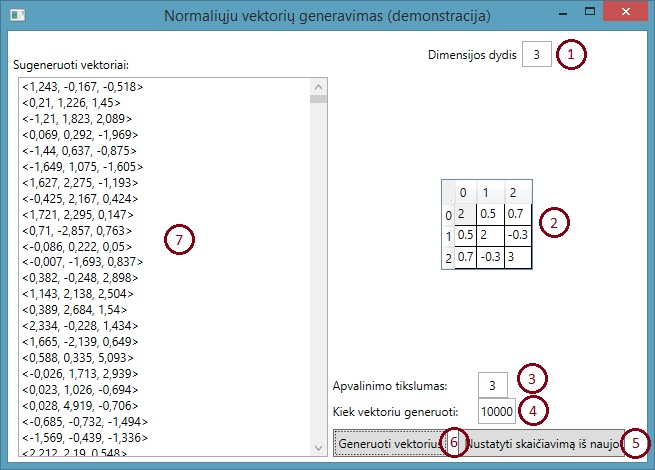
\includegraphics[width=13.5cm]{programa}\\

Trumpai galime pakomentuoti šios programos funkcionalumą.
Generuojame vektorių $\mathrm{y}=(y_1, \ldots, y_n)$:
\begin{enumerate}
	\item Galime numatyti kelių dimensijų vektorius programa generuos,
	
	\item Pateikiame matricą {\bf R}, verta pastebėti, kad matricos įstrižainės reikšmė $r_{ii}$ nurodo, kokia bus generuojamo vektoriaus $i-tosios$ dydžio standartinis nuokrypis $\sigma_i$, o matricos reikšmės $r_{ij}, \space i \neq j$ nurodo koreliaciją $\rho_{ij}$ tarp dydžių $y_i$ ir $y_j$, taip pat $r_{ij} = r_{ji}$,
	
	\item nurodome, kiek skaitmenų po kablelio turės vektoriaus $\mathrm{y}$ kintamieji dydžiai $(y_1, \ldots, y_n)$,
	
	\item nurodome, kiek vektorių bus sugeneruota,
	
	\item siekiant pakartoti (pseudo) atsitiktinę vektorių seką galime nustatyti sekos skaičiavimą iš naujo. Taip galima sugeneruoti visiškai identišką seką sugeneruotai anksčiau,
	
	\item paspaudus šį mygtuką pradedami generuoti vektoriai,
	
	\item laukas į kurį yra išvedami pagal mūsų pateiktus parametrus sugeneruoti vektoriai.
\end{enumerate}

\newpage

\begin{thebibliography}{99}
	\addcontentsline{toc}{section}{Literatūra}
	\bibitem {STEPANAUSKAS}
	prof. G. Stepanauskas, \textit{Monte Karlo Metodas}, \url{http://uosis.mif.vu.lt/~stepanauskas/MK/Monte%20Karlo%20metodas.pdf} 
	
	\bibitem {DEAK}	
	I. Deak, \textit{Random number generators and simulation}, Akademiai Kiado, Budapest, 1990, p.166-196.
	
\end{thebibliography} 


\end{document}